\documentclass[12pt]{article}
\usepackage{amsmath}
\usepackage{amssymb}
\usepackage{geometry}
\usepackage{enumerate}
\usepackage{natbib}
\usepackage{float}%稳定图片位置
\usepackage{graphicx}%画图
\usepackage[english]{babel}
\usepackage{a4wide}
\usepackage{indentfirst}%缩进
\usepackage{enumerate}%加序号
\usepackage{multirow}%合并行
\title{\large UM-SJTU JOINT INSTITUTE\\Data Structures and Algorithms\\(VP281)\\\ \\\ \\\ \\\ \\\ \\\ \\\ \\\ \\\ \\\ \\\
Programming Assignment\\\ \\\ Programming Assignment Five\\\ Graph Algorithms \\\ \\\ \\\ \\\ \\\ }
\author{Name: Pan Chongdan\\ID: 516370910121}
\date{Date: \today}

\begin{document}
\maketitle
\newpage
\section{Introduction}
The programming assignment asks us to implement a graph data structure using the adjacency list
representation.
\section{Code Appendix}
The appendix shows the cpp code for main project and time comparison.
The following part is for the main algorithm
\begin{figure}[H]
\centering
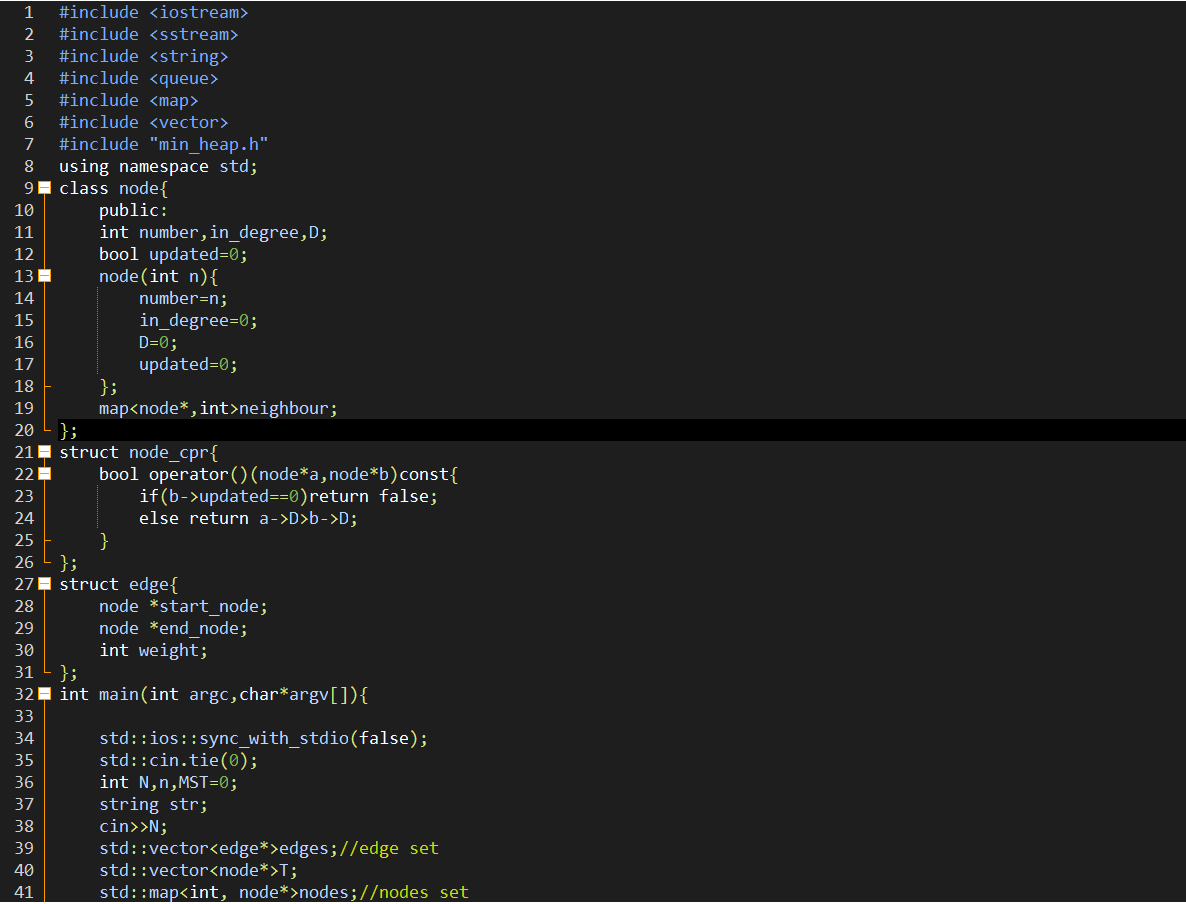
\includegraphics[scale=0.5]{1.png}
\end{figure}
\begin{figure}[H]
\centering
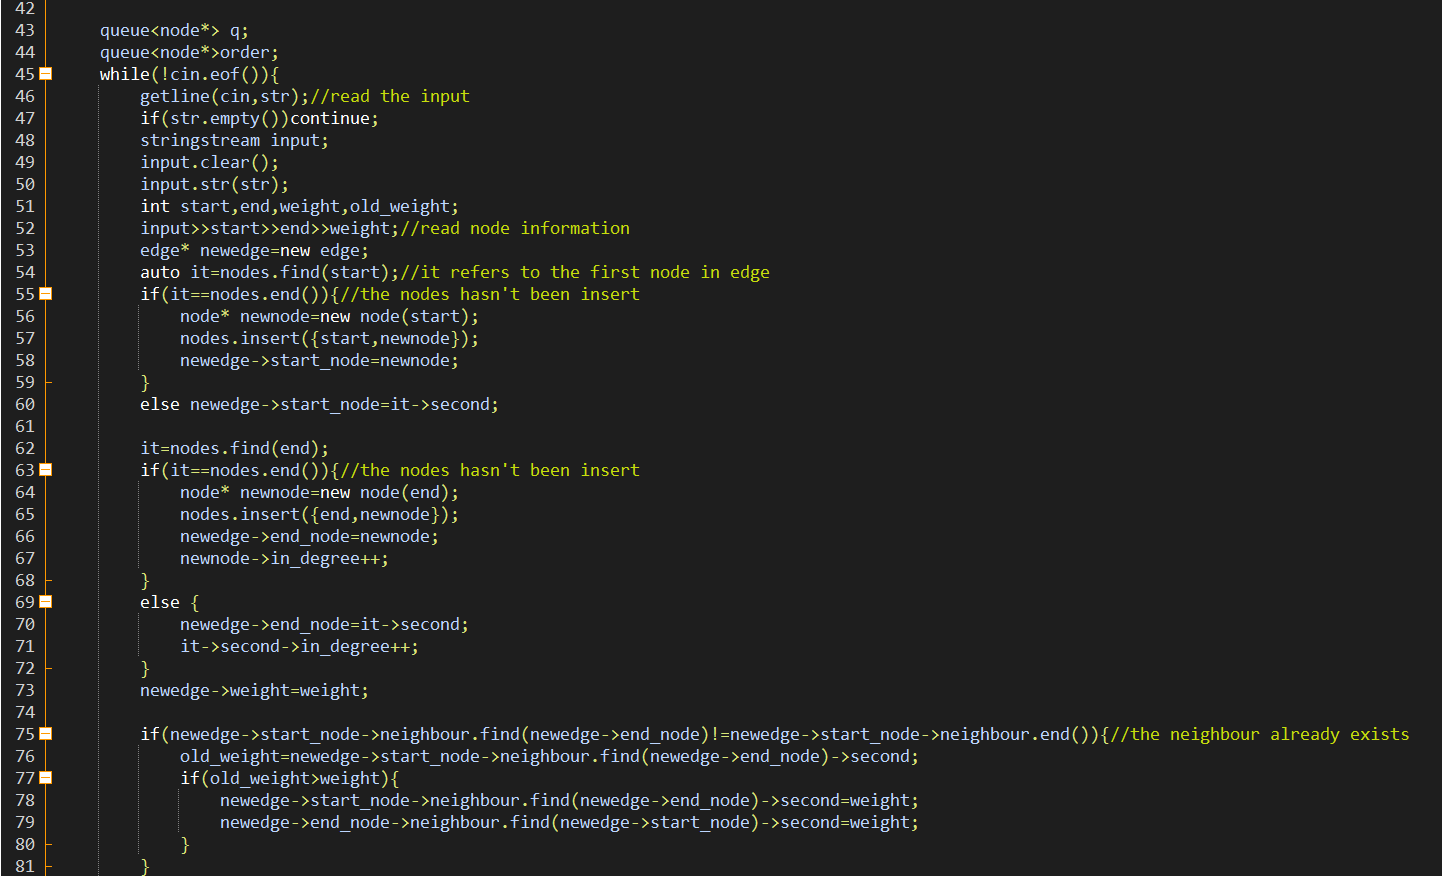
\includegraphics[scale=0.5]{2.png}
\end{figure}
\begin{figure}[H]
\centering
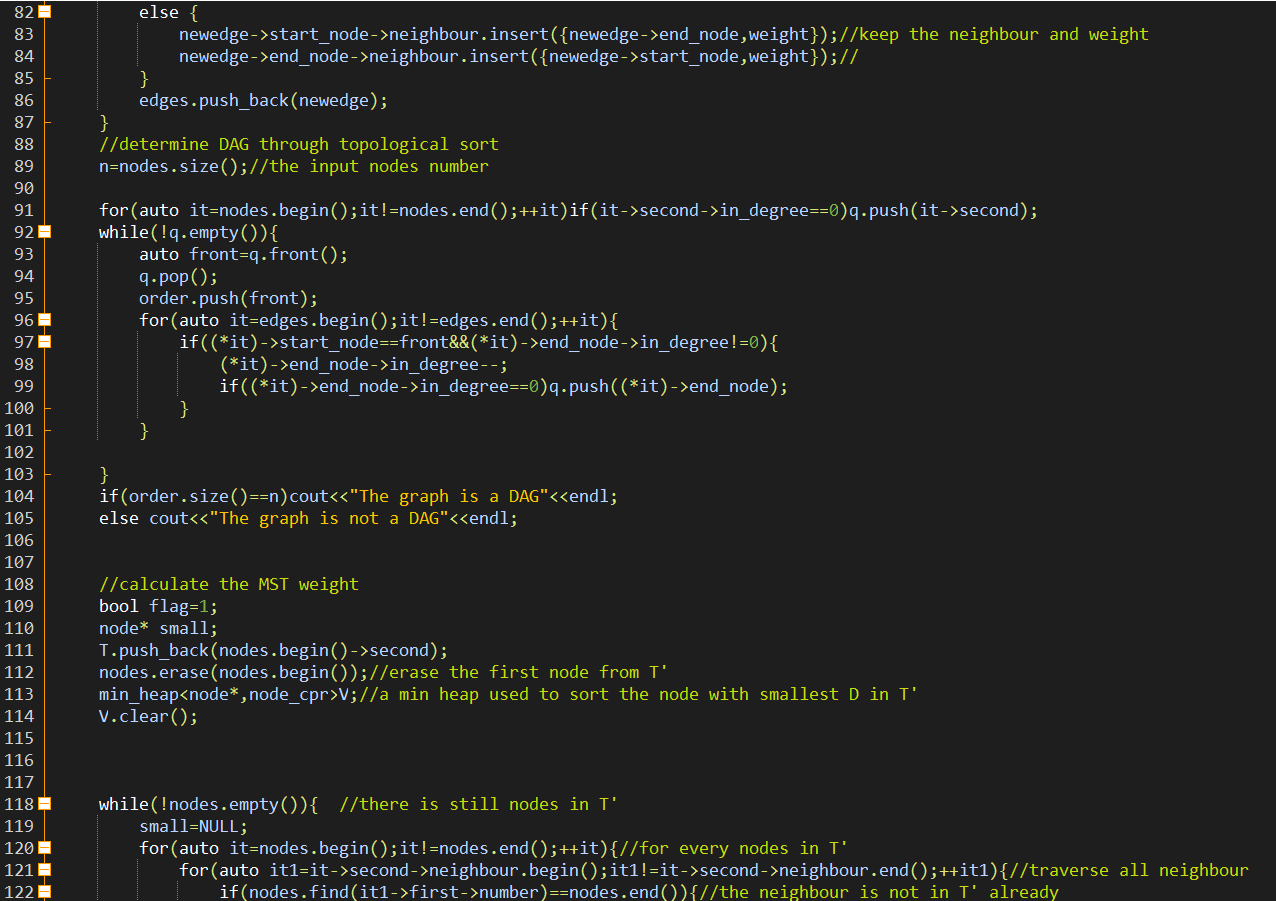
\includegraphics[scale=0.5]{3.png}
\end{figure}
\begin{figure}[H]
\centering
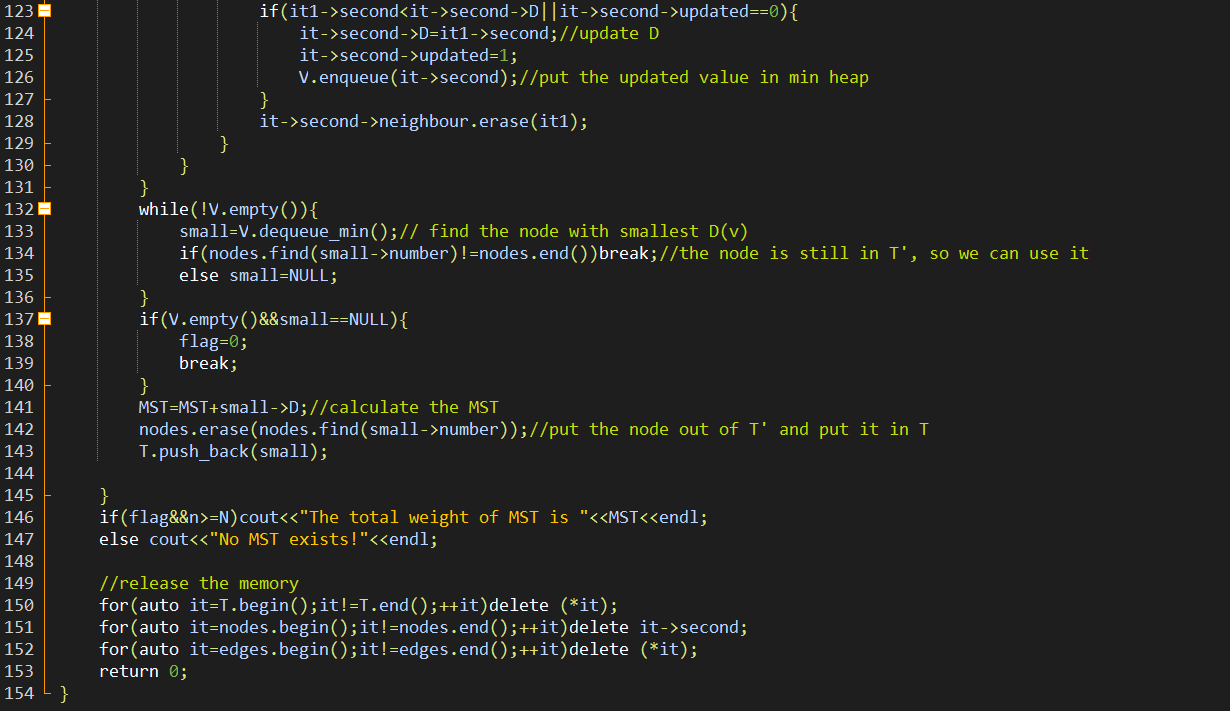
\includegraphics[scale=0.5]{4.png}
\end{figure}
The following is for min heap.
\begin{figure}[H]
\centering
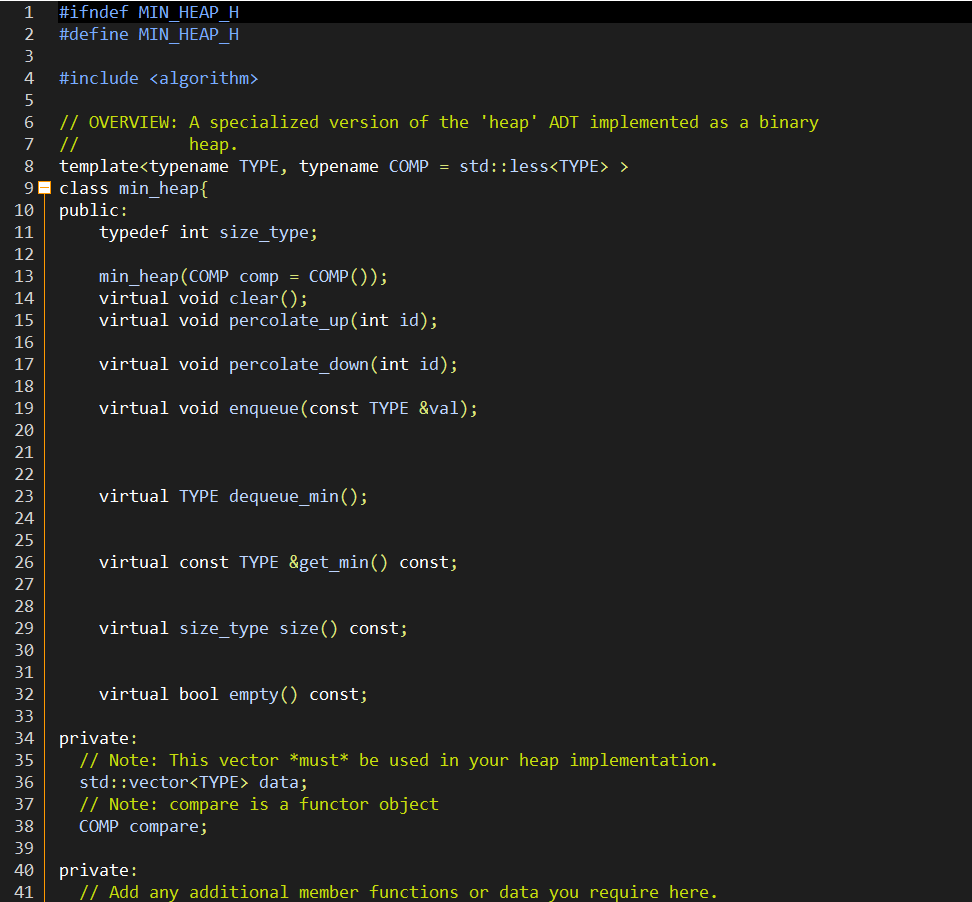
\includegraphics[scale=0.5]{5.png}
\end{figure}
\begin{figure}[H]
\centering
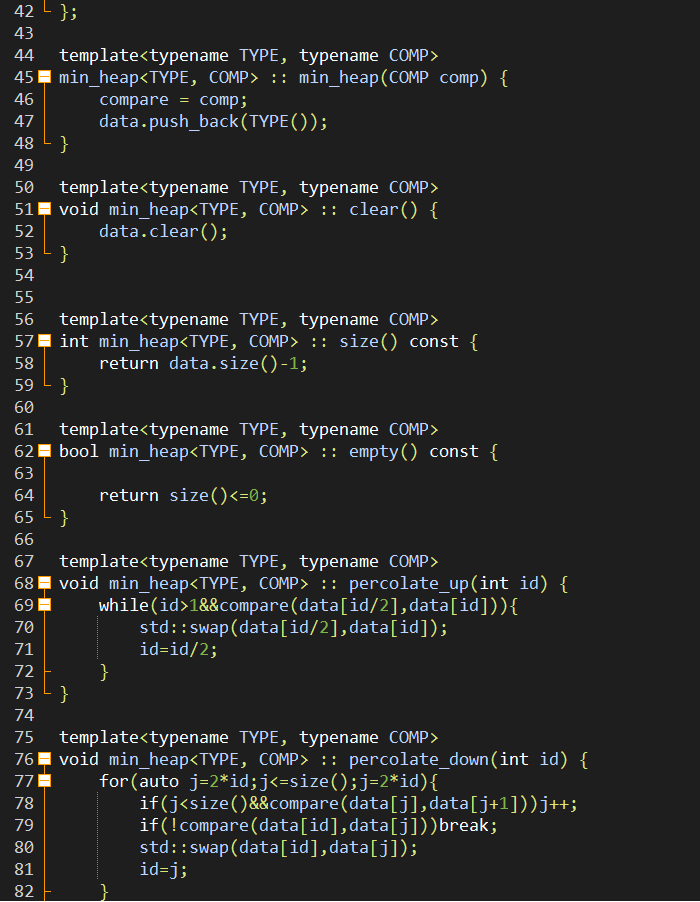
\includegraphics[scale=0.5]{6.png}
\end{figure}
The following is for unsorted heap.
\begin{figure}[H]
\centering
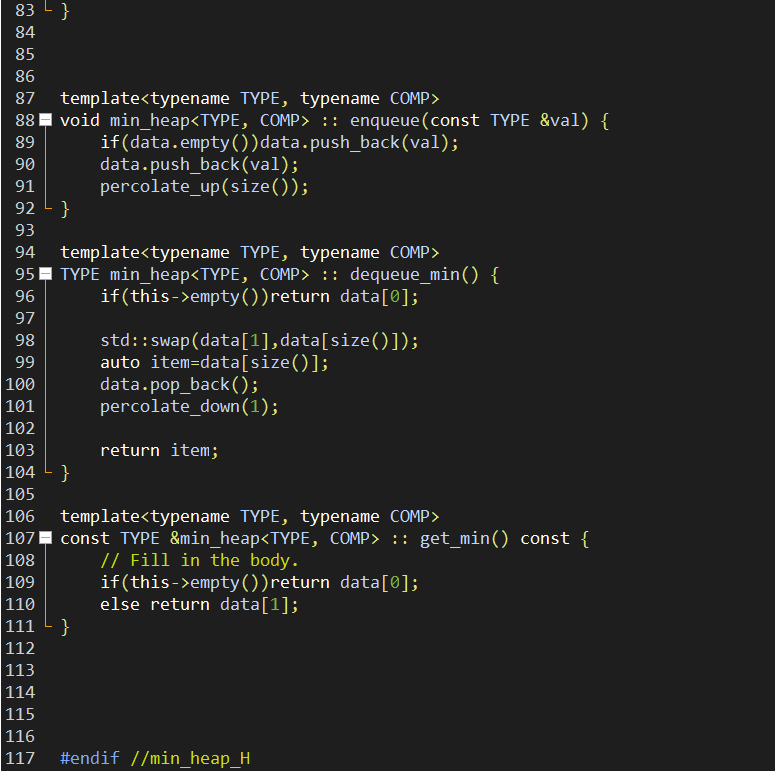
\includegraphics[scale=0.5]{7.png}
\end{figure}
\end{document}